\documentclass{article}
\usepackage[utf8]{inputenc}
\usepackage{tikz}
\usetikzlibrary{shapes,arrows}
\usepackage[ruled,vlined]{algorithm2e}
\usepackage{algpseudocode}
\usepackage{multicol}
\renewcommand{\contentsname}{{\Huge Table de Matières}}
\usepackage{titlesec}
\usepackage{xcolor}
\usepackage{listings}
\usepackage{graphicx}
\usepackage[normalem]{ulem}
\titleformat{\section}{\huge\bfseries}{\thesection}{1em}{}
\titleformat{\subsection}{\LARGE\bfseries}{\thesubsection}{1em}{}
\titleformat{\subsubsection}{\Large\bfseries}{\thesubsubsection}{1em}{}
\begin{document}
\begin{center}
\pagenumbering{gobble}
\linespread{2.0}\selectfont

{\Huge U}{\huge NIVERSITÉ DE }{\Huge M}{\huge ONTPELLIER}\\
{\huge L3}{\LARGE ~INFORMATIQUE }
\\~\\~\\~\\~\\
{\Large\textbf{TOURNOI SPORTIF\\"ESport"}}
\\~\\~\\~\\~\\

\linespread{1}\selectfont

RAPPORT DE PROJET\\~\\
PROJET INFORMATIQUE COMMUN AVEC\\
 HLIN510 ET HLIN511\\
\vfill
\end{center}
\begin{multicols}{2}
\begin{flushleft}
\textbf{GROUPE B}\\~\\
~~~M. Benjamin Baska\\~~~~~~~Numero etudiant: 21503576\\
~~~M. Kevin Lastra\\~~~~~~~Numero etudiant: 21706783\\
\end{flushleft}
\columnbreak
\begin{flushright}
\textbf{Enseignant responsable:}\\~\\
M. Pierre Pompidor~~~\\
M. Michele Meynard~~\\
M. Pascale Poncelet~~~
\end{flushright}
\end{multicols}
\newpage
\section{Modelé Entité/Association}

\begin{figure}[h]
\centering
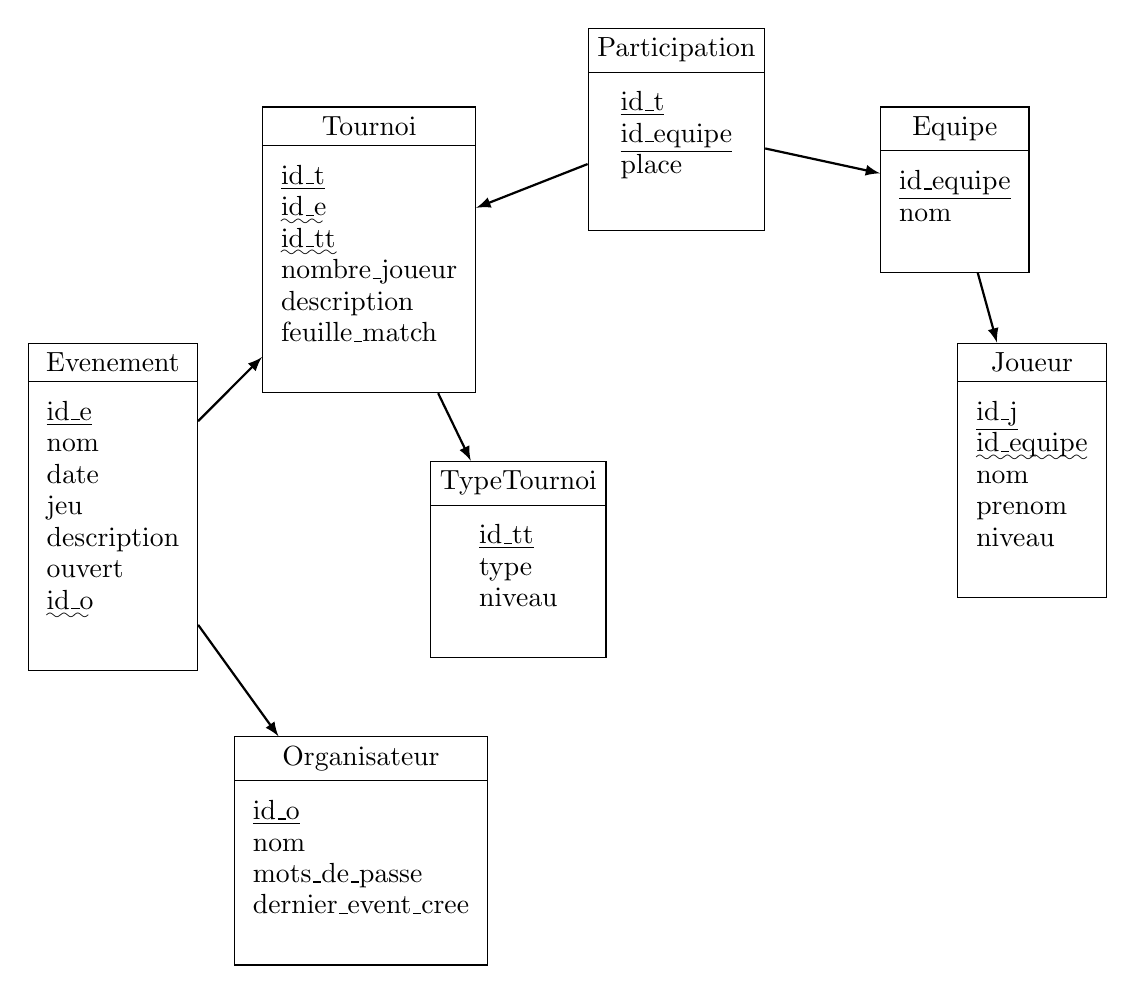
\begin{tikzpicture}[
					double/.style={draw, anchor=text, 		rectangle split, rectangle split parts=2},
					triple/.style={draw, anchor=text, rectangle split, rectangle split parts=3},
					triangle/.style={draw, shape=regular polygon, regular polygon sides=3,draw,thick,inner sep=0pt, minimum size=1cm, inner sep=-1.2cm, outer sep=0pt}]
					
    % Place nodes
    \node [double] (A) at (-6,0){Evenement
    	\nodepart{second}
    	\tikz{
    	\node at (0,0) {\underline{id\_e}};
    	\node at (0,-0.4) {nom};
    	\node at (0,-0.8) {date};
    	\node at (0,-1.2) {jeu};
    	\node at (0,-1.6) {description};
    	\node at (0,-2) {ouvert};
    	\node at (0,-2.4) {\uwave{id\_o}};
    }};
    \node [double] (B) at (1,4){Participation
    	\nodepart{second}
    	\tikz{
    	\node at (0,0) {\underline{id\_t}};
    	\node at (0,-0.4) {\underline{id\_equipe}};
    	\node at (0,-0.8) {place};
    }};
    \node [double] (C) at (-2.5,3){Tournoi
    	\nodepart{second}
    	\tikz{
    	\node at (0,0) {\underline{id\_t}};
    	\node at (0,-0.4) {\uwave{id\_e}};
    	\node at (0,-0.8) {\uwave{id\_tt}};
    	\node at (0,-1.2) {nombre\_joueur};
    	\node at (0,-1.6) {description};
    	\node at (0,-2) {feuille\_match};
    }};
    \node [double] (E) at (-3,-5){Organisateur
    	\nodepart{second}
    	\tikz{
    	\node at (0,0){\underline{id\_o}};
    	\node at (0,-0.4){nom};
    	\node at (0,-0.8){mots\_de\_passe};
    	\node at (0,-1.2){dernier\_event\_cree};
    }};
    \node [double] (F) at (5,3){Equipe
    	\nodepart{second}
    	\tikz{
		\node at (0,0) {\underline{id\_equipe}};
    	\node at (0,-0.4) {nom};
    }};
    \node [double] (G) at (-1,-1.5){TypeTournoi
    	\nodepart{second}
    	\tikz{
		\node at (0,0) {\underline{id\_tt}};
    	\node at (0,-0.4) {type};	 
    	\node at (0,-0.8) {niveau};	   	
    }};
    \node [double] (H) at (6,0){Joueur
    	\nodepart{second}
    	\tikz{
		\node at (0,0) {\underline{id\_j}};
		\node at (0,-0.4) {\uwave{id\_equipe}};
    	\node at (0,-0.8) {nom};	    	
    	\node at (0,-1.2) {prenom};	    
    	\node at (0,-1.6) {niveau};		
    }};
    \draw[thick,-latex] (A) edge (C);
    \draw[thick,-latex] (A) edge (E);
	\draw[thick,-latex] (B) edge (C);	
	\draw[thick,-latex] (C) edge (G);
	\draw[thick,-latex] (B) edge (F);
	\draw[thick,-latex] (F) edge (H);	
    % Draw edges
    
\end{tikzpicture}~\\

\end{figure}~\\

\noindent
\begin{tabular}{|c|l|l|}
\hline
Tables & Composant & Résumer\\
\hline
Evenement & id\_e & Clé primaire\\
& nom & Nom de l’événement\\
& date & Date de début de l’événement\\
& jeu & Jeu pour lequel est destinée l’événement\\
& description & Description de l’événement écrit par l'organisateur\\
& ouvert & Boolean contrôlant l'ouverture et fermeture de l’événement\\
& id\_o & Clé étrangère pour organisateur\\
\hline
Organisateur & id\_o & Clé primaire\\
& nom & Nom d'utilisateur de l'organisateur\\
& mot\_de\_passe &  Mot de passe de l'organisateur\\
& dernier\_event\_cree & Dernière date à laquelle l'organisateur a crée un événement\\
\hline
Tournoi & id\_t & Clé primaire\\
& id\_e & Clé étrangère pour événement\\
& id\_tt & Clé étrangère pour TypeTournoi\\
& nombre\_joueur & Nombre maximum d'équipe dans un tournoi\\
& description & Description du tournoi écrit par l'organisateur\\
& feuille\_match & Format de text (JSON) pour sauvegarde les brackets\\
\hline
TypeTournoi & id\_tt & Clé primaire\\
& type & Format de compétition des équipes, \{1v1, 2v2, ...\}\\
& niveau & Niveau du tournoi a titre indicatif\\
\hline
Participation & id\_t & Clé primaire et Clé étrangère pour Tournoi\\
& id\_equipe & Clé primaire et Clé étrangère pour Equipe\\
& place & Position final dans le tournoi\\
\hline
Equipe & id\_equipe & Clé primaire\\
& nom & Nom de l'équipe\\
\hline
Joueur & id\_j & Clé primaire\\
& id\_equipe & Clé étranger pour équipe\\
& nom & Nom du joueur\\
& prenom & Prénom du joueur\\
& niveau & Niveau du joueur indiquée par lui-même\\
\hline
\end{tabular}
\\
\newpage

\section{Modelé Relationnel}

{\large\parindent 1pt
evenement(\underline{id\_e}, nom, date, jeu, description, ouvert, \uwave{id\_o})\\~

participation(\underline{id\_equipe},\underline{id\_t}, place)\\~

tournoi(\underline{id\_t}, \uwave{id\_tt}, \uwave{id\_e}, nombre\_joueur, description, feuille\_match)\\~

typetournoi(\underline{id\_tt}, type, niveau)\\~

equipe(\underline{id\_equipe}, nom)\\~

joueur(\underline{id\_j}, \uwave{id\_equipe}, nom, prenom, niveau)\\~

organisateur(\underline{id\_o} , nom, mot\_de\_passe, dernier\_event\_cree)\\~
}
\section{Procédures Fonctionnels}
Renvoi tout les évènement de l'organisateur passer en paramètre.
\begin{verbatim}
CREATE PROCEDURE event_par_org (IN org_id INT)
BEGIN
    SELECT e.id_e, e.nom
    FROM evenement e
    WHERE e.id_o = org_id;
END
\end{verbatim}
~\\
Renvoi les stats d'un évènement passer en paramètre.
\begin{verbatim}
CREATE PROCEDURE stats_event(IN event_id INT)
BEGIN
    SELECT e.id_e, e.nom, e.id_o, o.nom, COUNT(t.id_t)
    FROM evenement e, tournoi t, organisateur o
    WHERE e.id_e = event_id AND e.id_o = o.id_o AND t.id_e = event_id
    GROUP BY e.id_e;
    
    SELECT t.id_t, COUNT(e.id_equipe)
    FROM equipe e, tournoi t, participation p
    WHERE t.id_e = event_id AND p.id_t = t.id_t AND p.id_equipe = e.id_equipe
    GROUP BY t.id_t;
END
\end{verbatim}
\section{Triggers}
Quand un organisateur crée un évènement la date du dernier évènement crée est actualiser a la date actuelle.
\begin{verbatim}
CREATE TRIGGER update_organisateur_last_date AFTER INSERT ON evenement
FOR EACH ROW
BEGIN
    UPDATE organisateur
    SET dernier_event_cree = CURDATE()
    WHERE id_o = NEW.id_o;
END;
\end{verbatim}
~\\
Quand un organisateur est supprimer, tout les évènement a son nom et changer pour l'organisateur para default "root".
\begin{verbatim}
CREATE TRIGGER delete_organisateur BEFORE DELETE ON organisateur
FOR EACH ROW
BEGIN	
    UPDATE evenement SET id_o = 1
           WHERE id_o = OLD.id_o;
END;
\end{verbatim}
\end{document}